\section{Schaltende Regler \formelbuch{61}}
Bei schaltenden Reglern dagegen enthalten die Signale u und y wenig Information, im Extremfall nur 1 Bit. Die Stellgrösse kann zwei Werte annehmen und die Strecke 'auf die eine oder andere Seite' beeinflussen. Umgekehrt gibt der Sensor durch zwei Werte an, 'auf welcher Seite' sich der Prozess befindet. Ein zu schnelles Hin- und Herschalten des Reglers wird oft durch eine Hysterese verhindert. Bsp. Temperaturregelung Bügeleisen. 

	\subsection{Zweipunktregler \formelbuch{63}}
		\begin{minipage}{5cm}
 		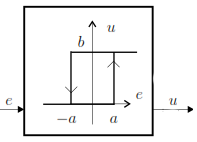
\includegraphics[height=3cm]{./bilder/Zweipunkteregler.png}
        \end{minipage}
		\begin{minipage}{12cm}
        Ein Zweipunktregler ist ein unstetig arbeitender Regler mit zwei Ausgangszuständen. Je nachdem, ob der Istwert über oder unter dem Sollwert liegt, wird der erste oder der zweite Ausgangszustand eingenommen. 
        \end{minipage}
	
	\subsubsection{Beispiele von Zweipunkte-Reglerschaltungen:}
		\textbf{Zweipunktregler mit symmetrischer Kennlinie \formelbuch{52}} \\
		\begin{minipage}{9cm}
			\vspace{.5cm}        
	 		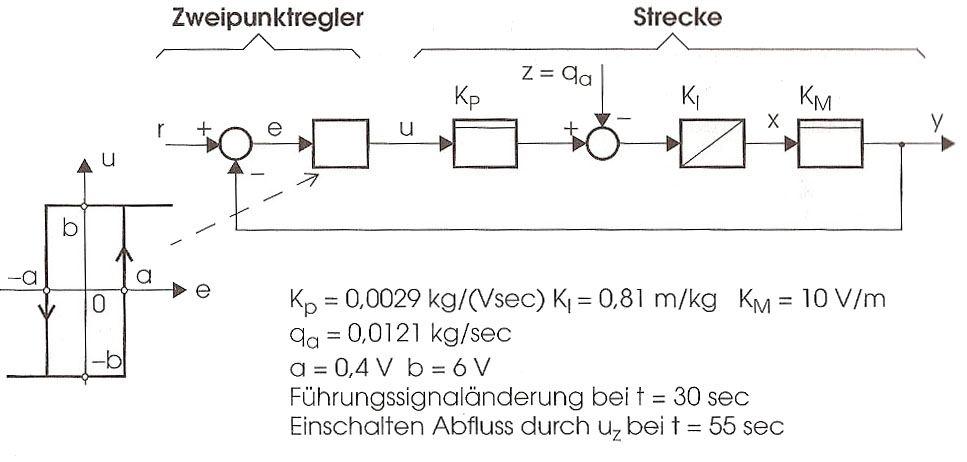
\includegraphics[width=9cm]{./bilder/Zweipunktregler-b+b2.jpg}\\
			Die Anstiegszeit beträgt nach dem Einschwingvorgang:\\
			$t_{ein}=\frac{2a}{(b K_p - q_a)K_i K_m}$ \\ \\
			Die Abfallszeit beträgt nach dem Einschwingvorgang:\\
			$t_{aus}=\frac{2a}{(b K_p + q_a)K_i K_m}$
        \end{minipage}
		\begin{minipage}{9cm}
			\vspace{.5cm}        
			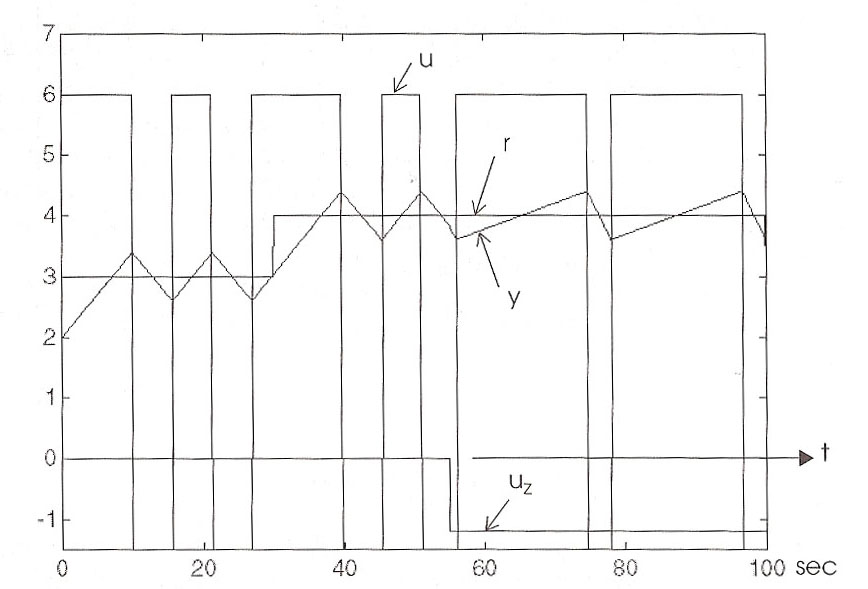
\includegraphics[width=9cm]{./bilder/Zweipunktregler-b+b_dia.jpg}
        \end{minipage}\\
         Einfüllen mit Abfluss: $y = y_0 + K_M \cdot K_I(K_p \cdot b - Q_a)(t-t_0); \qquad$ 
         Entleeren: $y=y_1 + K_M \cdot K_I(K_p(-b) - Q_a)(t-t_0)$
    
	\vspace{.5cm}
		\textbf{Zweipunktregler an ausgleichender Strecke \formelbuch{53}} \\
		\begin{minipage}{9cm}
 		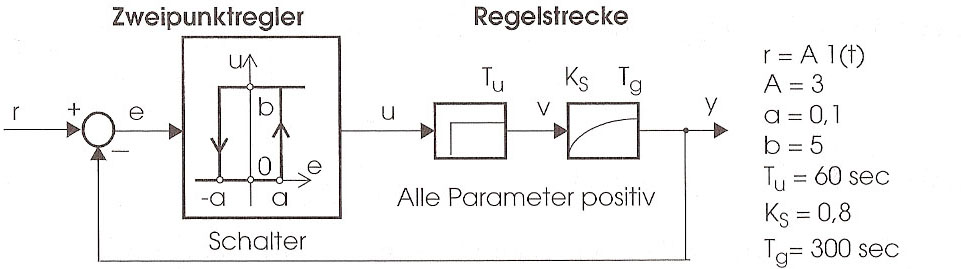
\includegraphics[width=9cm]{./bilder/ZweipunktreglerTotglied2.jpg}\\
			Die Anstiegszeit beträgt nach dem Einschwingvorgang:
			$t_{ein}$=$T_g\ln(\frac{e^{-\frac{T_u}{T_g}}(A-a)-b K_s}{A+a-b K_s})+T_u$\\ \\
			Die Abfallszeit beträgt nach dem Einschwingvorgang:
			$t_{aus}$=$T_g\ln(\frac{A+a-b
			K_s+\frac{b K_s}{e^{-\frac{T_u}{T_g}}}}{A-a})$\\
        \end{minipage}
		\begin{minipage}{9cm}
		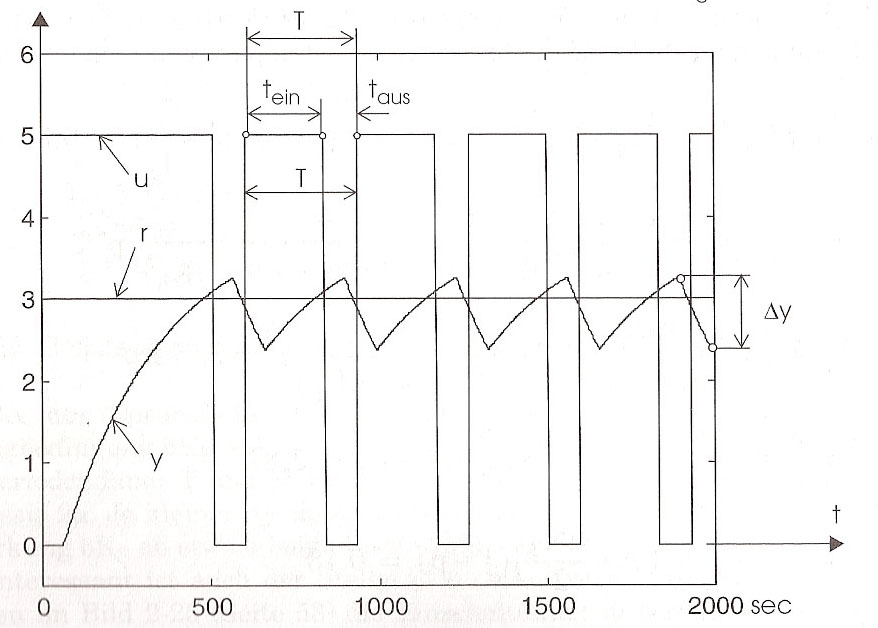
\includegraphics[width=9cm]{./bilder/ZweipunktreglerTotglied_dia.jpg}			
        \end{minipage}
    
 	$\Delta y = b\cdot K_s - e^{-\frac{T_u}{T_G}}(b\cdot K_s - 2a); \qquad$
	$y_m = \frac{y_{min}+y_{max}}{2}=e^{-\frac{T_u}{T_G}}\cdot A + \frac{b\cdot K_s}{2}(1-e^{-\frac{T_u}{T_G}}$
\newpage


\subsection{Dreipunktregler \formelbuch{70}}		
\begin{minipage}{5cm}
 		\includegraphics[height=3cm]{./bilder/Dreipunktregler1.png}
\end{minipage}
		\begin{minipage}{14cm}
        Ein Dreipunktregler ist ein unstetig arbeitender Regler mit drei Ausgangszuständen. Je nachdem, ob der Istwert unter dem ersten Sollwert, zwischen erstem und zweitem Sollwert, oder über dem zweiten Sollwert liegt, wird der erste, zweite oder dritte Ausgangszustand eingenommen. Dreipunktregler kommen dann zum Einsatz, wenn die Stellgrösse nicht stetig variabel ist. 
        \end{minipage}
       
		